\documentclass[18pt]{beamer}
\usepackage[utf8]{inputenc} % for the umlauts
\usepackage{subfigure}

\beamertemplatenavigationsymbolsempty
%% SLIDE FORMAT

% use 'beamerthemekit' for standard 4:3 ratio
% for widescreen slides (16:9), use 'beamerthemekitwide'

\usepackage{templates/beamerthemekit}
% \usepackage{templates/beamerthemekitwide}

\setcounter{tocdepth}{1}

%% TITLE PICTURE

% if a custom picture is to be used on the title page, copy it into the 'logos'
% directory, in the line below, replace 'mypicture' with the 
% filename (without extension) and uncomment the following line
% (picture proportions: 63 : 20 for standard, 169 : 40 for wide
% *.eps format if you use latex+dvips+ps2pdf, 
% *.jpg/*.png/*.pdf if you use pdflatex)

%\titleimage{mypicture}

%% TikZ INTEGRATION

% use these packages for PCM symbols and UML classes
% \usepackage{templates/tikzkit}
% \usepackage{templates/tikzuml}

% the presentation starts here

\usepackage{mathabx}
\usepackage{picture}
\usepackage[absolute,overlay]{textpos}
\usepackage{csquotes}
%\usepackage[texcoord,grid,gridunit=mm,gridcolor=red, subgridcolor=green]{eso-pic}
\setbeamercovered{invisible}
\setbeamertemplate{caption}{\raggedright\insertcaption\par}

\title[SWT1]{Softwaretechnik 1 - 6. Tutorium}
\subtitle{Tutorium 17}
\author{Felix Bachmann}
\date{23.07.2019}
\institute{KIT - Institut für Programmstrukturen und Datenorganisation (IPD)}


\begin{document}
	
% change the following line to "ngerman" for German style date and logos
\selectlanguage{ngerman}
\setcounter{tocdepth}{2}
	
%title page
\begin{frame}
\titlepage
\end{frame}

\begin{frame}
\tableofcontents
\end{frame}


\section{Orga}
	\begin{frame}
		\frametitle{Termine}
		\begin{block}{Klausur, Übungsschein}
			\begin{itemize}
				\item Hauptklausur am 01.08.19, 11:00
				\item Nachklausur wahrscheinlich am 07.10.19
				\item Anmeldung sollte nun für alle möglich sein
			\end{itemize}
		\end{block}
	\end{frame}

	\begin{frame}
		\frametitle{Nicht abgeholte Übungsblätter}
		\begin{itemize}
			\item bringe ich zu den Übungsleitern (R346, in der Nähe vom Holzkasten)
			\begin{itemize}
				\item siehe \url{https://ps.ipd.kit.edu/3273.php}
			\end{itemize}
			\item falls ihr die noch haben wollt, holt sie euch dort ab
			\item Übungsleiter beißen (meistens) nicht
		\end{itemize}
	\end{frame}

	\subsection{Feedback}
	\begin{frame}
		\frametitle{6. Übungsblatt Statistik}
		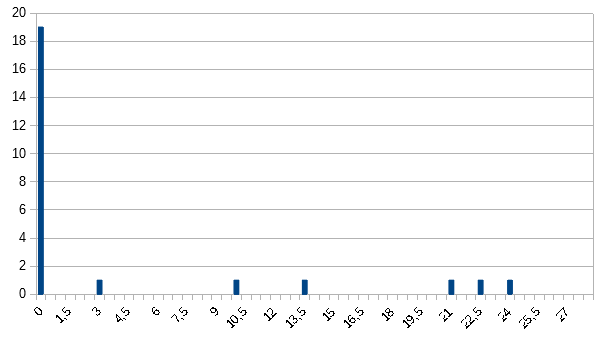
\includegraphics[scale=0.7]{./pics/tut6/statistics-ub6.png}
	\end{frame}

	\begin{frame}[fragile]
		\frametitle{Häufige Fehler}
		\begin{block}{Aufgabe 1: Kontrollfluss-orientiertes Testen}
			\begin{itemize}
				\pause 
				\item alles außer Kontrollfluss-Zeug so lassen wie es ist! \pause
				\item Kontrollfluss-Zeug, das nicht if(x) goto ist auflösen! \pause
				\item außerdem Kurzschlussauswertung in zwei if auflösen 
			\end{itemize}
		\end{block}
		\begin{verbatim}
		if(x && y) {
		  z++;
		}
		
		if(x || y) {
		  z++;
		}
		\end{verbatim}
\end{frame}

	\begin{frame}
		\frametitle{KFO: Kurzschlussauswertung}
		\begin{itemize}
			\item Kurzschlussauswertung (\&\& bzw. $\Vert$) muss berücksichtigt werden \pause
			\item Erinnerung: 
			\begin{itemize}
				\item \&\& und $\Vert$ werten die rechte Seite nur aus, wenn notwendig
				\item \& und $\vert$ werten immer beide Seiten aus \pause
			\end{itemize}
		\end{itemize}
		\centering 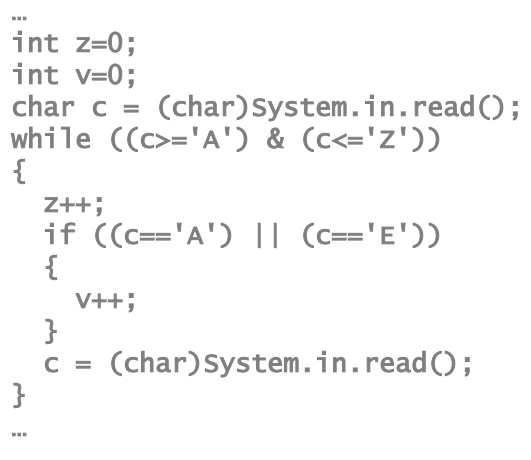
\includegraphics[scale=0.4]{./pics/tut6/code.png}
	\end{frame}

	\begin{frame}
		\frametitle{KFO: Kurzschlussauswertung}
		\begin{figure}
			\subfigure[1. Zwischensprache]{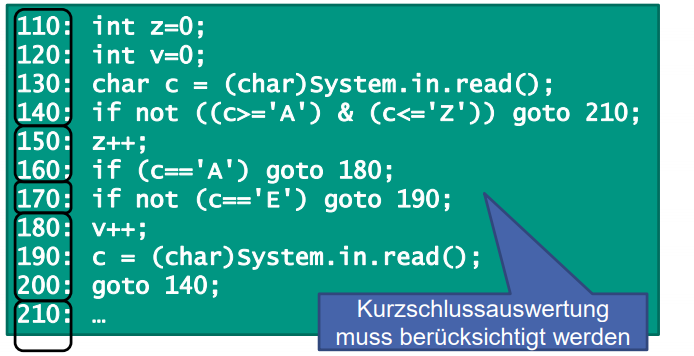
\includegraphics[scale=0.35]{./pics/tut6/zwischen.png}}	
			\subfigure[KFG]{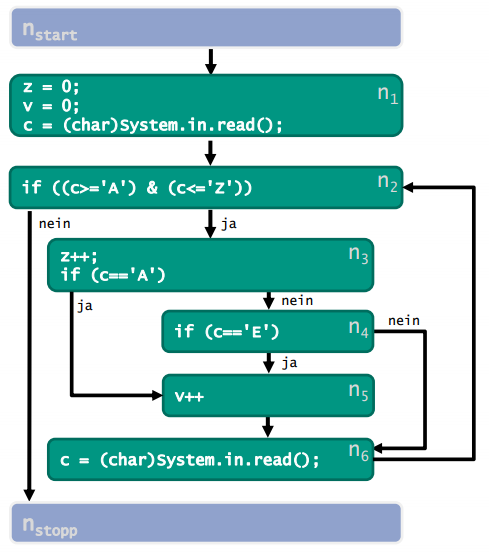
\includegraphics[scale=0.35]{./pics/tut6/kfg.png}}
		\end{figure}
	\end{frame}

	\begin{frame}
		\frametitle{Häufige Fehler}
		\begin{block}{Aufgabe 2: Parallelisierung}
			\begin{itemize}
				\item 5 Abgaben, meist richtig \pause
				\item Anzahl Prozessoren berechnen
				\begin{itemize}
					\item \texttt{int nproc = Runtime.getRuntime().availableProcessors();}
				\end{itemize}
			\end{itemize}
			\end{block}
		\pause 
		\begin{block}{Aufgabe 3: Abnahmetests}
			\begin{itemize}
				\item 4 Abgaben
				\item Test brauchen immer Asserts!
			\end{itemize}
		\end{block}
	\end{frame}

	\begin{frame}
		\frametitle{Häufige Fehler}
		\begin{block}{Aufgabe 4: Wettbewerb}
			\begin{itemize}
				\item 3 Abgaben
			\end{itemize}
		\end{block}
	\end{frame}
		
\section{Testen}
	\subsection{Definitionen}
	
	\begin{frame}
		\frametitle{Arten von Fehlern}
		\begin{itemize}
			\item Was verursacht was?
			\item Defekt, Irrtum, Versagen \pause
			\item Irrtum (Aktion) $\rightarrow$ Defekt (Bug) $\rightarrow$ Ausfall (failure)
			\item dumme Eselsbrücke: IDA
			\pause
			\item \enquote{Testing shows the presence of bugs, not their absence.} (Edsger W. Dijkstra)
		\end{itemize}
	\end{frame}

	\begin{frame}
		\frametitle{Arten von Tests}
		\begin{block}{Dynamische Verfahren}
			\begin{itemize}
				\item Testfälle schreiben und ausführen (z.B. mit JUnit) \pause
				\item white box testing \pause
				\begin{itemize}
					\item kontrollflussorientiert
					\item datenflussorientiert
				\end{itemize}
				\item black box testing \pause
				\begin{itemize}
					\item funktionale Tests \pause
					\item Leistungstests
				\end{itemize}
			\end{itemize}
		\end{block}
		\pause
		\begin{block}{Statische Verfahren}
			\begin{itemize}
				\item Inspektion (\enquote{scharfes Hinsehen}, Code Review, etc.)\pause
				\item statische Analyse mit Tools (formale Verifikation, SpotBugs, etc.)\pause
				\item Programm wird nicht ausgeführt!
			\end{itemize}
		\end{block}
	\end{frame}

\section{Wiederholung und Klausuraufgaben}

	\subsection{Planung \& Definition}
	\begin{frame}
		\frametitle{Disclaimer}
		\begin{large}
			\begin{itemize}
				\item Ich kenne die Klausur auch nicht! \pause
				\linebreak $\implies$ alles, was ich zum Inhalt der Klausur sage ist Spekulation
				\begin{itemize}
					\item basierend auf Altklausuren \pause
				\end{itemize}
				\item kein Anspruch auf Vollständigkeit der Wiederholung
			\end{itemize}
		\end{large}
	\end{frame}

	\begin{frame}
		\frametitle{Die typische SWT-Klausur}
		\begin{enumerate}
			\item Aufgabe 1: Aufwärmen
			\begin{itemize}
				\item Wahr-/Falsch-Fragen 
				\begin{itemize}
					\item ein paar gesammelt auf \url{www.github.com/malluce/swt1-tut/multiple_choice.txt}
				\end{itemize} 
				\item Wissensfragen 
			\end{itemize} 
			\pause
			\item meistens Aufgaben zu:
			\begin{itemize}
				\item UML-Diagrammen \pause
				\item Entwurfsmustern \pause
				\item Parallelität \pause
				\item Testen bzw. Qualitätssicherung (KFG!) \pause
				\item Rest (z.B. Objektorientierung, Git/Versionskontrolle, Prozessmodelle\dots)
			\end{itemize}
		\end{enumerate}
		\pause 
		\begin{itemize}
			\item bisher: $\frac{1}{3} \pm \epsilon$ der Punkte reichen zum Bestehen
			\begin{itemize}
				\item kann sich eventuell ändern, wegen längerer Bearbeitungszeit
			\end{itemize}
		\end{itemize}
	\end{frame}

	\begin{frame}
		\frametitle{Aufwärmaufgabe}
		\begin{huge}
			\centering Hauptklausur SS2011 A1
		\end{huge}
	\end{frame}

	\begin{frame}
		\frametitle{Planung \& Definition}
		\begin{itemize}
			\item Lastenheft, Pflichtenheft \pause
			\begin{itemize}
				\item Phasen zuordnen \pause
				\item Gliederung kennen \pause
				\item Beispiele geben \pause
			\end{itemize}
			\item UML-Diagramme \pause
			\begin{itemize}
				\item Klassendiagramm \pause
				\item Aktivitäts-, Sequenz-, Zustandsdiagramm \pause 
				\item Anwendungsfalldiagramm \pause
				\item Syntax kennen! \pause
				\item gegebenen Text/Code in Diagramm umwandeln \pause
				\item bei Zustandsdiagramm
				\begin{itemize}
					\item Umwandeln hierarchisch $\Leftrightarrow$ nicht-hierarchisch 
					\item Umwandeln parallel $\Leftrightarrow$ nicht-parallel
				\end{itemize}
			\end{itemize}
		\end{itemize}
	\end{frame}

	\begin{frame}
		\frametitle{Zustandsdiagramm-Aufgabe}
		\begin{huge}
			 	\centering Hauptklausur SS2012 A2
		\end{huge}
	\end{frame}

	\subsection{Entwurf}
	\begin{frame}
		\frametitle{Entwurf}
		\begin{itemize}
			\item Architekturstile \pause
			\item \textbf{Entwurfsmuster} \pause
			\begin{itemize}
				\item möglichst viele, bestenfalls alle kennen und verstehen \pause
				\item Kategorien kennen \pause
				\item Klassendiagramm hinzeichnen (auch auf Szenario angepasst) \pause
				\item aus Klassendiagrammen/Code Entwurfsmuster erkennen \pause
				\item Code für Muster schreiben \pause
				\item Code-Schnipsel auf mögliche Verbesserung durch EM untersuchen
			\end{itemize}
		\end{itemize}
	\end{frame}

	\begin{frame}
		\frametitle{Entwurfsmuster-Aufgabe}
		\begin{huge}
				\centering Hauptklausur SS2010 A3
		\end{huge}
	\end{frame}

	
	\subsection{Implementierung}
	\begin{frame}
		\frametitle{Implementierung}
		\begin{itemize}
			\item UML-Abbildung \pause
			\item \textbf{Parallelität} \pause
			\begin{itemize}
				\item grundlegendes Prinzip \pause
				\item in Java \pause
				\item critical sections/ race conditions \pause
				\item deadlock \pause
				\item Monitore, wait \& notify \pause
				\item Semaphore \pause
			\end{itemize}
			\item Rechnungen können (Speedup, Amdahls Law (\textbf{Tafel})) \pause
			\item gegebenen Code thread-safe machen \pause
			\item Lösungsvorschläge zur Synchronisation bewerten \pause
			\item eigenen Code schreiben
		\end{itemize}
	\end{frame}

	\begin{frame}
		\frametitle{Parallelität-Aufgabe}
		\begin{huge}
				\centering Hauptklausur SS2011 A3
		\end{huge}
	\end{frame}
	
	\subsection{Testen}
	\begin{frame}
		\frametitle{Testen}
		\begin{itemize}
			\item Testphasen 
			\begin{itemize}
				\item Komponententest, Integrationstest, Systemtest, Abnahmetest \pause
			\end{itemize}
			\item Testverfahren
			\begin{itemize}
				\item \textbf{Kontrollflussgraph} \pause \textbf{\underline{!!!}}
				\begin{itemize}
					\item absolute Standardaufgabe \pause
					\item in 33 von 36 der letzten Altklausuren
					\item in allen Klausuren seit SS14
					\item im Schlaf können ("'Schema F"', lässt sich sehr gut üben\dots)
				\end{itemize}
			\end{itemize} \pause
			\item Testhelfer
			\item Definitionen kennen (Fehlerarten\dots)
		\end{itemize}
	\end{frame}

	\begin{frame}
	\frametitle{KFG: Klausuraufgabe}
	\begin{huge}
		\centering Hauptklausur SS2016 A6
	\end{huge}
	\end{frame}
	
	\subsection{Abnahme, Einsatz \& Wartung}
	\begin{frame}
		\frametitle{Abnahme, Einsatz \& Wartung}
		\begin{itemize}
			\item Aufgaben der verschiedenen "'Subphasen"' kennen \pause
			\item viel Text zum Lernen, aber nicht schwierig\dots \pause
			\item Wartung vs. Pflege \pause
			\item selten eigene Aufgabe dazu, eher Ankreuzaufgaben in A1
		\end{itemize}
	\end{frame}

	\subsection{Rest}
	\begin{frame}
		\frametitle{Rest}
		\begin{itemize}
			\item Schätzmethoden \pause
			\item Prozessmodelle \pause
			\item Agile Prozesse \pause
			\item verschiedene Modelle kennen (XP, Scrum,\dots) \pause
			\item auch eher Ankreuzaufgaben, Wissensfragen
		\end{itemize}
	\end{frame}

	\begin{frame}{Git: Klausuraufgabe}
		\begin{huge}
			\centering Hauptklausur SS18 A4
		\end{huge}
	\end{frame}

	\begin{frame}{Git: Klausuraufgabe}
		\centering 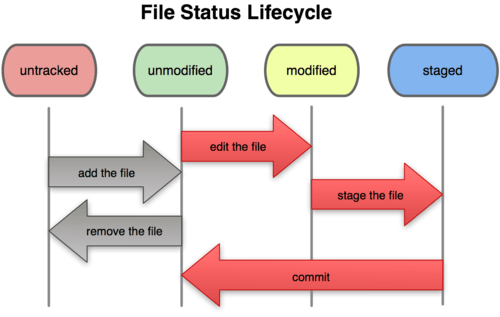
\includegraphics[width=100mm, scale=1.3]{./pics/tut0/git-file-lifecycle.png}
	\end{frame}

	\begin{frame}
		\frametitle{Backup: Klassendiagramm-Aufgabe}
		\begin{huge}
			\centering Nachklausur SS2011 A5
		\end{huge}
	\end{frame}

\section{Ende}
	\subsection{Feierabend}
	\begin{frame}
		\frametitle{Lernen}
		\begin{itemize}
			\item Klausuren rechnen \texttt{\&\&} Folien anschauen
			\begin{itemize}
				\item Übung nötig, für sehr gute Note aber auch viel Wissen
			\end{itemize}
		\pause
			\item diesmal habt ihr mehr Zeit für den gleichen Umfang an Aufgaben wie in früheren Klausuren
			\begin{itemize}
				\item vermutlich wird Bestehensgrenze hochgesetzt
			\end{itemize}
		\end{itemize}
	\end{frame}

	\begin{frame}{Das war's dann wohl\dots}
		\begin{itemize}
			\item danke für Eure Anwesenheit und Mitarbeit!
			\item Viel Erfolg bei der Klausur und im weiteren Studium! :)
		\end{itemize}
	\end{frame}

	\begin{frame}
		\centering

		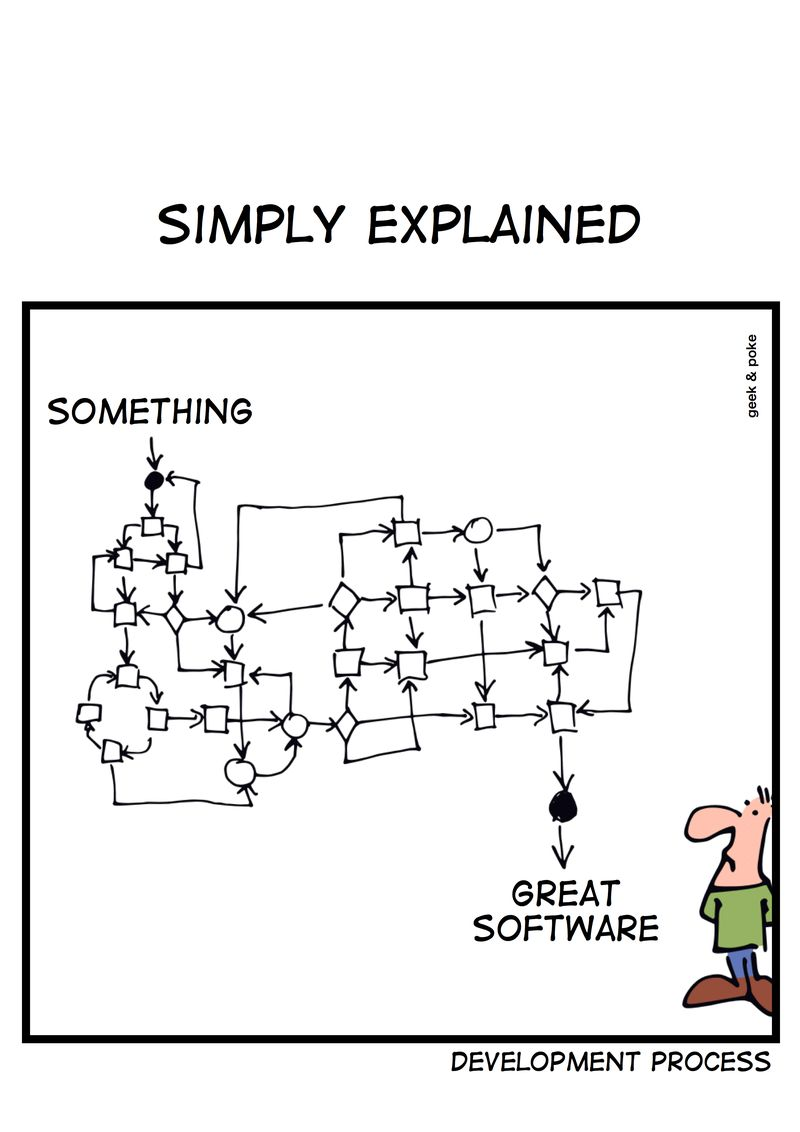
\includegraphics[scale=0.9]{./comics/geek_and_poke_development2.jpg}
	\end{frame}

\end{document}